
\subsection{Primer diseño}

A partir de una selección del video proporcionada por el usuario se obtienen las mejores features del objeto seleccionado utilizando el algoritmo de Shi-Tomasi. Luego, mediante el algoritmo de Lucas-Kanade de Optical Flow se obtiene la evolución de dichas features en el tiempo. A este cúmulo de puntos se le calcula el centro de masas $\mu$ y el centro de inercia $\sigma$. Se rechazan los puntos de este cúmulo que se encuentren a una distancia mayor a $k_{\sigma}\sigma$ respecto al centro de masas, para luego calcular nuevamente el centro de masas el cual es el que se introduce en el filtro de Kalman como medición de la posición.

La dimensión del vector de estados del filtro de Kalman es de cuatro, poseyendo la posición y la velocidad tanto horizontal como vertical. La dimensión del vector de observación es de dos dado que solamente se mide la posición horizontal y vertical del centro de masas. La matriz $A$ queda definida por las ecuaciones que caracterizan el movimiento del objeto a seguir que, por simplicidad, se consideraron las ecuaciones cinemáticas de MRU, quedando entonces
\begin{equation}
\begin{pmatrix} x_{k-1} + dt\cdot v_{x_{k-1}} \\y_{k-1} + dt\cdot v_{y_{k-1}} \\ v_{x_{k-1}}  \\ v_{y_{k-1}} \end{pmatrix} =\begin{pmatrix}
1 & 0 & dt  & 0\\
0 & 1  & 0 & dt\\
0 & 0  & 1  & 0\\
0 & 0  & 0  & 1 
\end{pmatrix} \cdot \begin{pmatrix} x_{k-1}\\y_{k-1} \\ v_{x_{k-1}}  \\ v_{y_{k-1}} \end{pmatrix}
\end{equation}
Siendo, 
\begin{equation}
A = 
\begin{pmatrix}
1 & 0 & dt  & 0\\
0 & 1  & 0 & dt\\
0 & 0  & 1  & 0\\
0 & 0  & 0  & 1 
\end{pmatrix}
\end{equation}

Luego, se tiene que la matriz de observación o de transición de medición quedará definida por la transformación del espacio de observación al espacio real del vector de estados del filtro. Como los observables a medir forman parte del espacio real del vector de estados y son solo las posiciones, la matriz quedará definida de manera simple
\begin{equation}
\begin{pmatrix} z_{x_{k}} \\ z_{y_{k}} \end{pmatrix}=\begin{pmatrix}
1 & 0 & 0  & 0\\
0 & 1  & 0 & 0  \end{pmatrix} \cdot  \begin{pmatrix} x_k \\ y_k \\ v_{x_{k}} \\ v_{y_{k}}
\end{pmatrix}
\end{equation}
Siendo,
\begin{equation}
H = 
\begin{pmatrix}
1 & 0 & 0  & 0\\
0 & 1  & 0 & 0 
\end{pmatrix}
\end{equation}

Mientras que la matrices de covarianza del proceso $Q$ y de medición $R$ serán cuadradas por definición, de dimensión cuatro y dos respectivamente, y además de la forma $\mathbb{I}\cdot \xi$ dado que se asume independencia de las variables aleatorias, quedando

\begin{equation}
Q = 
\begin{pmatrix}
\xi_Q & 0 & 0  & 0\\
0 & \xi_Q  & 0 & 0\\
0 & 0  & \xi_Q  & 0\\
0 & 0  & 0  & \xi_Q 
\end{pmatrix}
\end{equation}

\begin{equation}
R = 
\begin{pmatrix}
\xi_R & 0 \\
0 & \xi_R 
\end{pmatrix}
\end{equation}

Siendo $\xi_Q$ y $\xi_R$ las varianzas del proceso y de medición respectivamente.

Finalmente, $\hat{x}_{k|k}$ y $P_{k|k}$ tomarán la forma

\begin{equation}
\hat{x}_{k|k} = 
\begin{pmatrix}
\hat{x}\\
\hat{y}\\
\hat{v_x}\\
\hat{v_y}
\end{pmatrix}
\end{equation}

\begin{equation}
P_{k|k} = 
\begin{pmatrix}
\gamma_{x} & 0 & 0  & 0\\
0 & \gamma_{y}  & 0 & 0\\
0 & 0  & \gamma_{v_x}  & 0\\
0 & 0  & 0  & \gamma_{v_y} 
\end{pmatrix}
\end{equation}

Siendo $\gamma_{i}$ la varianza de cada variable de estado. Cabe notar que el modelo utilizado asume independencia entre las variables aleatorias por simplicidad.

Este algoritmo, hasta ahora explicado, cuenta con grandes problemas. Dados dos objetos $A$ y $B$, donde $A$ es el objeto a seguir:

\begin{itemize}
\item Como el algoritmo de Shi-Tomasi tiende a colocar features en bordes bien definidos, y estos suelen ser los bordes externos de un objeto, si el objeto a seguir $A$ pasa por delante de un objeto $B$ con bordes bien definidos, las features del algoritmo de Optical Flow tenderán a adosarse a los bordes del objeto $B$ por más que este esté quieto.
\item Si el objeto $A$ pasase por detrás del objeto $B$ inmóvil, todas las features sobre el objeto a seguir quedarían adosadas al objeto $B$. Esto plantea un problema mucho más grande que el anterior, dado que no se podrá utilizar la estimación del filtro de Kalman de manera confiable, debido a que cuando los features se queden quietos adosados en $B$, se seguirá midiendo de todas formas y se seguirán entregando esas mediciones al filtro de Kalman, por lo que la estimación de este se adosará también al objeto $B$.
\item Profundizando en el item anterior, existe una ambigüedad entre que $A$ pase de un movimiento MRU a que se quede completamente quieto y que $A$ pase por detras de $B$, dado que en ambas situaciones las features quedarán quietas en el lugar donde $A$ se haya quedado quieto o el lugar de la intersección entre $A$ y $B$
\end{itemize}

\subsection{Segundo diseño}

La mejora propuesta para sortear estos problemas consiste en agregar un filtro de color, para diferenciar a $A$ y a $B$ por su color. La implementación de este filtro de color comienza en el momento en el que el usuario selecciona el área a seguir. Se calcula la mediana del color de la zona elegida, y ese color es transformado de formato RGB a formato HSV, o Hue-Saturation-Value, dado que es más sencillo definir una máscara de este modo. Dado $x$ e $y$ las coordenadas de los píxeles de la imagen, $\vec{R_k}$, $\vec{G_k}$ y $\vec{B_k}$ los vectores de píxeles de la selección, $mediana(\vec{R_k}, \vec{G_k}, \vec{B_k}) = (m_R, m_G, m_B)$ el vector que define la mediana del color de la selección, $\mathbb{HSV}$ el operador de transformación del espacio de coordenadas RGB a HSV, y $\mathbb{HSV}(m_R, m_G, m_B) = (m_H, m_S, m_V)$ el vector de la mediana del color de la selección en el espacio HSV, queda entonces definida la máscara de color como

\begin{equation}
f(x, y) = (f_h(x, y), f_s(x, y), f_v(x, y))
\end{equation}

\begin{equation}
f_{u}(x,y) = \left\{
\begin{array}{ll}


      1 & -\Lambda_u < u_{x, y} - m_u < \Lambda_u \\
      
      
      
      0 & \text{sino} \\
      
      
\end{array} 
\right.
\end{equation}

donde $\Lambda$ es el límite para cada propiedad $u$, siendo estas Hue, Saturation o Value. Una vez obtenida la máscara $f(x, y)$ se realiza la operación AND entre la máscara y la imagen original, logrando obtener una intensidad nula en los píxeles de la imagen que no posean un color cercano a la mediana calculada como se puede ver en las Figuras (\ref{fig:col1}) y (\ref{fig:col2}).

\begin{figure}[H]
\centering
	\begin{subfigure}{.4\textwidth}
		\centering
		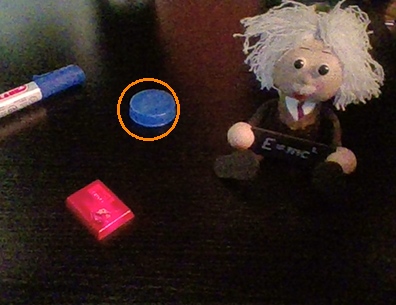
\includegraphics[width=\textwidth]{Imagenes/color1.png}
		\caption{Video antes de aplicar la máscara siguiendo al objeto azul.}
		\label{fig:col1}
	\end{subfigure}
	\begin{subfigure}{.4\textwidth}
		\centering
		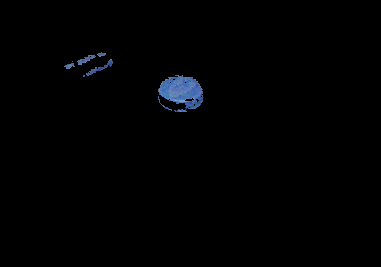
\includegraphics[width=\textwidth]{Imagenes/color2.png}
		\caption{Video después de aplicar la máscara. Es con esta imagen que opera el algoritmo y no con la normal.}
		\label{fig:col2}
	\end{subfigure}
	\caption{Comparación entre video normal y luego de aplicar la máscara.}
	\label{fig:color_comp}
\end{figure}

Este filtrado de color no solo posee una gran sinergia con el método de obtención de features de Shi-Tomasi, dado que este frame tendrá bordes de mucha mejor calidad, sino que también posee una gran sinergia con el método de Optical Flow, debido a que como se verán menos bordes en la imagen modificada, aumenta notablemente la probabilidad de que los features queden contenidos todos dentro, o sobre los bordes del objeto a seguir.

Volviendo al caso de los objetos $A$ y $B$:

\begin{itemize}
\item Si $A$ y $B$ son de colores distintos, con el filtro de color, el algoritmo nunca detectará que existe un objeto $B$ por lo que seguirlo será imposible, y por consecuencia seguirá únicamente a $A$ y no se tendrá el problema de $A$ pasando por frente de $B$.
\item Si $A$ y $B$ son de colores distintos, y $A$, el objeto a seguir, pasa por detrás de $B$, ahora no se adosarán las features al objeto $B$, sino que el algoritmo verá que el área de $A$ se achica a medida que este queda oculto por $B$. Como los features no tendrán bordes para seguir, estos desaparecerán, por lo que se dejará de entregar mediciones al filtro de Kalman y este estimará correctamente la posición de $A$ mientras que este no haya sufrido aceleración alguna mientras estaba oculto. 
\end{itemize}

\begin{figure}[H]
\centering
	\begin{subfigure}{.4\textwidth}
		\centering
		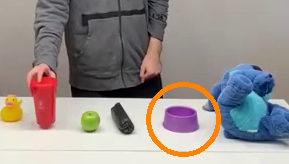
\includegraphics[width=\textwidth]{Imagenes/Optical1.png}
		\caption{Ventana con el funcionamiento normal del seguidor, el cual utiliza un círculo naranja para detallar donde se encuentra el objeto a seguir.}
		\label{fig:optical1}
	\end{subfigure}
	\begin{subfigure}{.4\textwidth}
		\centering
		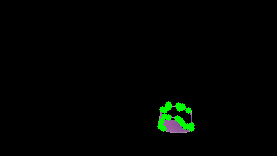
\includegraphics[width=\textwidth]{Imagenes/Optical2.png}
		\caption{Ventana la cual solo aparece al seleccionar el modo debug. Aquí se muestra si el filtro de color se encuentra activado, el video luego de pasar por la máscara de color, las features del objeto como puntos verdes y la zona de búsqueda si se diese el caso de tracking failure.}
		\label{fig:optical2}
	\end{subfigure}
	\caption{Resultado de la selección de un elemento.}
	\label{fig:optical12}
\end{figure}

Sin embargo, el filtro de Kalman no puede estimar la posición del objeto indefinidamente. Es por esto que cuando el objeto se pierde, es decir, no se logran detectar más features, se entra en otra fase del programa. En esta fase, se realiza una búsqueda del objeto en cada frame del video a partir de la estimación del filtro de Kalman y el tamaño original del área seleccionada. La altura y el ancho del área de búsqueda se incrementará por un factor constante por cada frame en la que la búsqueda falle. Esta búsqueda se basa en aplicar el algoritmo de Shi-Tomasi sobre el área mencionada.


Finalmente, para reforzar el algoritmo de seguimiento, se implemento además una recalculación periódica de las features con el método de Shi-Tomasi, partiendo de la media del cúmulo de features, removiendo los outliers, volviendo a calcular nuevamente la media y utilizar esta posición para aplicar el algoritmo de Shi-Tomasi, de misma manera que se realiza sobre la primera selección proporcionada por el usuario. Todo esto nos permite subsanar varios de los problemas planteados anteriormente, sin embargo, existen aún varios otros problemas:

\subsection{Escenarios de fallas}
Algunos casos donde puede fallar hasta ahora el Tracker son:
\begin{itemize}
\item El cambio de trayectoria de un objeto una vez que desaparece, provocará una falla en la predicción.
\item Interacción entre el objeto trackeado y un objeto de características similares, puede causar un error de detección
\item Cambios bruscos de iluminación o en color del objeto.
\end{itemize}

\subsection{Último diseño}

\begin{figure*}
\centering
	\includegraphics[width=0.9\textwidth]{../flowchart.jpg}
	\caption{Flow-chart del algoritmo.}
	\label{fig:Flowchart}
\end{figure*}


\begin{figure}
\centering
	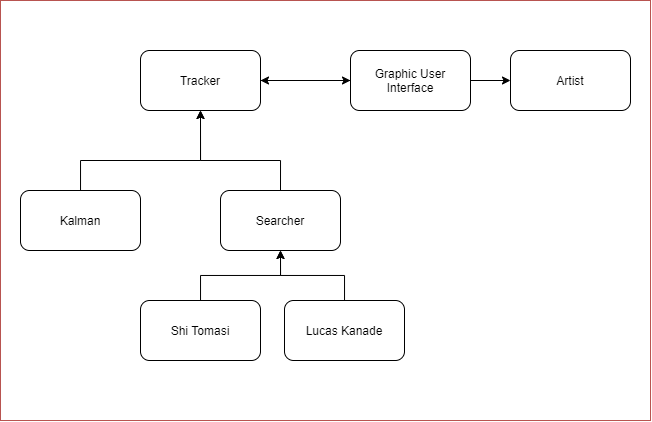
\includegraphics[width=0.5\textwidth]{Imagenes/classd.png}
	\caption{Diagrama de Clases del programa utilizado para presentar la funcionalidad del algoritmo desarollado.}
	\label{fig:class}
\end{figure}
EXPLICAR LO SIGUIENTE
\begin{itemize}
\item Filtro de color pasó del espacio HSV a CIE-LAB, explicar que es para mas invarianza a la iluminacion
\item Al filtro de color se le unió una alternativa, el de camshift, explicar en qué situaciones es mejor uno o el otro
\end{itemize}

\subsection{Algoritmo correlación}
Para el algoritmo de correlación no solo se utiliza el filtro explicado en la sección \ref{sec:corr}, sino que ademas se trata tanto al frame como al kernel, aplicando una transformación al espacio \textbf{HSV} y allí un filtrado bajo las siguientes especificaciones: 
            
\begin{align}
MSK = H \  \epsilon \ (0,180 ) \ \ S \  \epsilon \ (50,255) \ \ V \ \epsilon \ (32,255)
\end{align}
Una vez que se hace esto se utiliza el filtro de correlación y se obtiene el punto donde esta es mayor, se toma una sección al rededor de este punto proporcional a la selección inicial y se compara con el frame original, si no comparte las características de color que son calculadas por el filtrado de color, este punto de correlación es desechado. Esto se logra aplicando una máscara en la sección del frame de mayor correlación, sobre este se realiza nuevamente el cálculo de máxima correlación, este proceso se realizan unas pocas veces con el propósito de no comprometer la velocidad de procesamiento entre frames. En caso de no encontrar al objeto se considera que hubo un error de trackeo (Oclusión del objeto).\\

\begin{figure}[H]
\centering

		\begin{subfigure}{.5\textwidth}
		\centering
		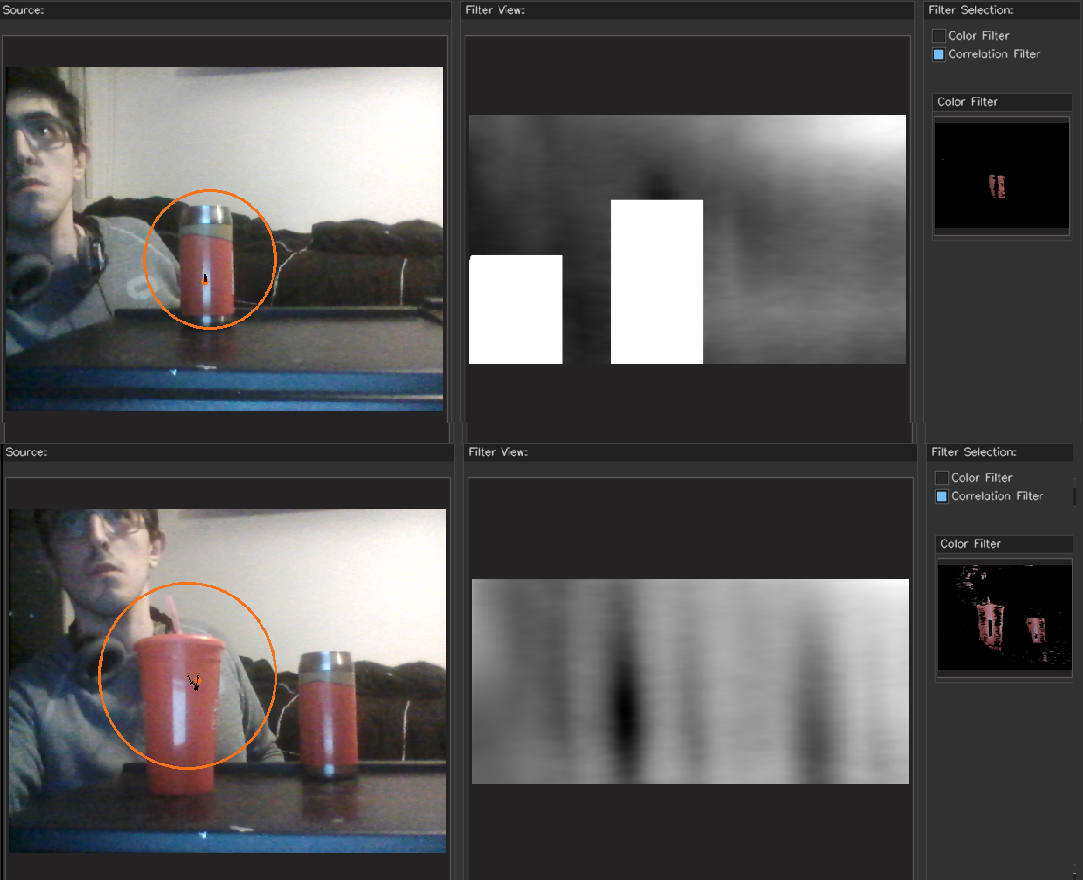
\includegraphics[width=1\textwidth]{Imagenes/corrmask.png}
		\caption{Correlación con máscara ante oclusión del objeto}
		\label{fig:sqdiff}
	\end{subfigure}
	\begin{subfigure}{.1\textwidth}
		\centering
		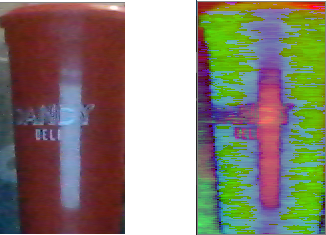
\includegraphics[width=1\textwidth]{Imagenes/kernelhsv.png}
		\caption{Kernel}
		\label{fig:kernel}
	\end{subfigure}
	\caption{Aplicación del algoritmo de correlación con máscara.}
	\label{fig:corrtest}
\end{figure}

Este algoritmo es utilizado en dos escenarios, para la búsqueda de un objeto perdido, en el caso de oclusión se  utiliza el algoritmo para encontrar nuevamente el objeto, este es efectivo siempre que no haya objetos que compartan tanto forma y color con el de interés, en el caso de que así sea y el objeto de interés se encuentre oculto es posible que el algoritmo devuelva un falso positivo, en ese caso conviene utilizar el alternativo de Shi-Tomasi y medias móviles, dado que el tener información de la posición previa para el tracking resulta fundamental para poder distinguir entre estos.
Otro escenario es  utilizar la correlación para el recálculo periódico de features, esto es beneficioso en el caso de la interacción de dos objetos $A$ y $B$ siendo $A$ el de interés y $B$ uno similar, si $B$ pasa por delante de $A$ quitandole las features, el cálculo periódico por correlación podrá detectar que se está siguiendo a $B$ y no a $A$ por lo que corregirá este error. Una situación similar a esta no puede ser resuelta por el algoritmo de Shi-Tomasi con medias móviles.


\subsection{Optimización del Código}
Se realizó una optimización del código, quitando redundancias y utilizando únicamente librerías que son corridas en C++ con la finalidad de que el procesamiento en tiempo real sea eficiente. Se optó por un enfoque OOP, esto permitió escalar el proyecto y obtener una mayor modularidad. \\
Además se diseñó una GUI con la capacidad de trackeo multi-objeto, personalización de algoritmos, contando con la opcion de variar algoritmos tanto de búsqueda como de recáclculo entre medias móviles y correlación, al giaul que filtrado por color o camshift, teniendo la opción de cambiar las especificaciones de los filtros en tiempo real para obtener el filtro óptimo. También se permite diversas pantallas de debug, al igual que una estimación de la posición y velocidad del objeto, finalmente cuenta con la capacidad de utilizar tanto un video en tiempo real como un video pre-existente.





% Finalmente se presenta un diagrama en bloques del programa, donde se puede apreciar como interaccionan todos %los algoritmos trabajando en armonía.
%\begin{figure}[H]
%\centering
%	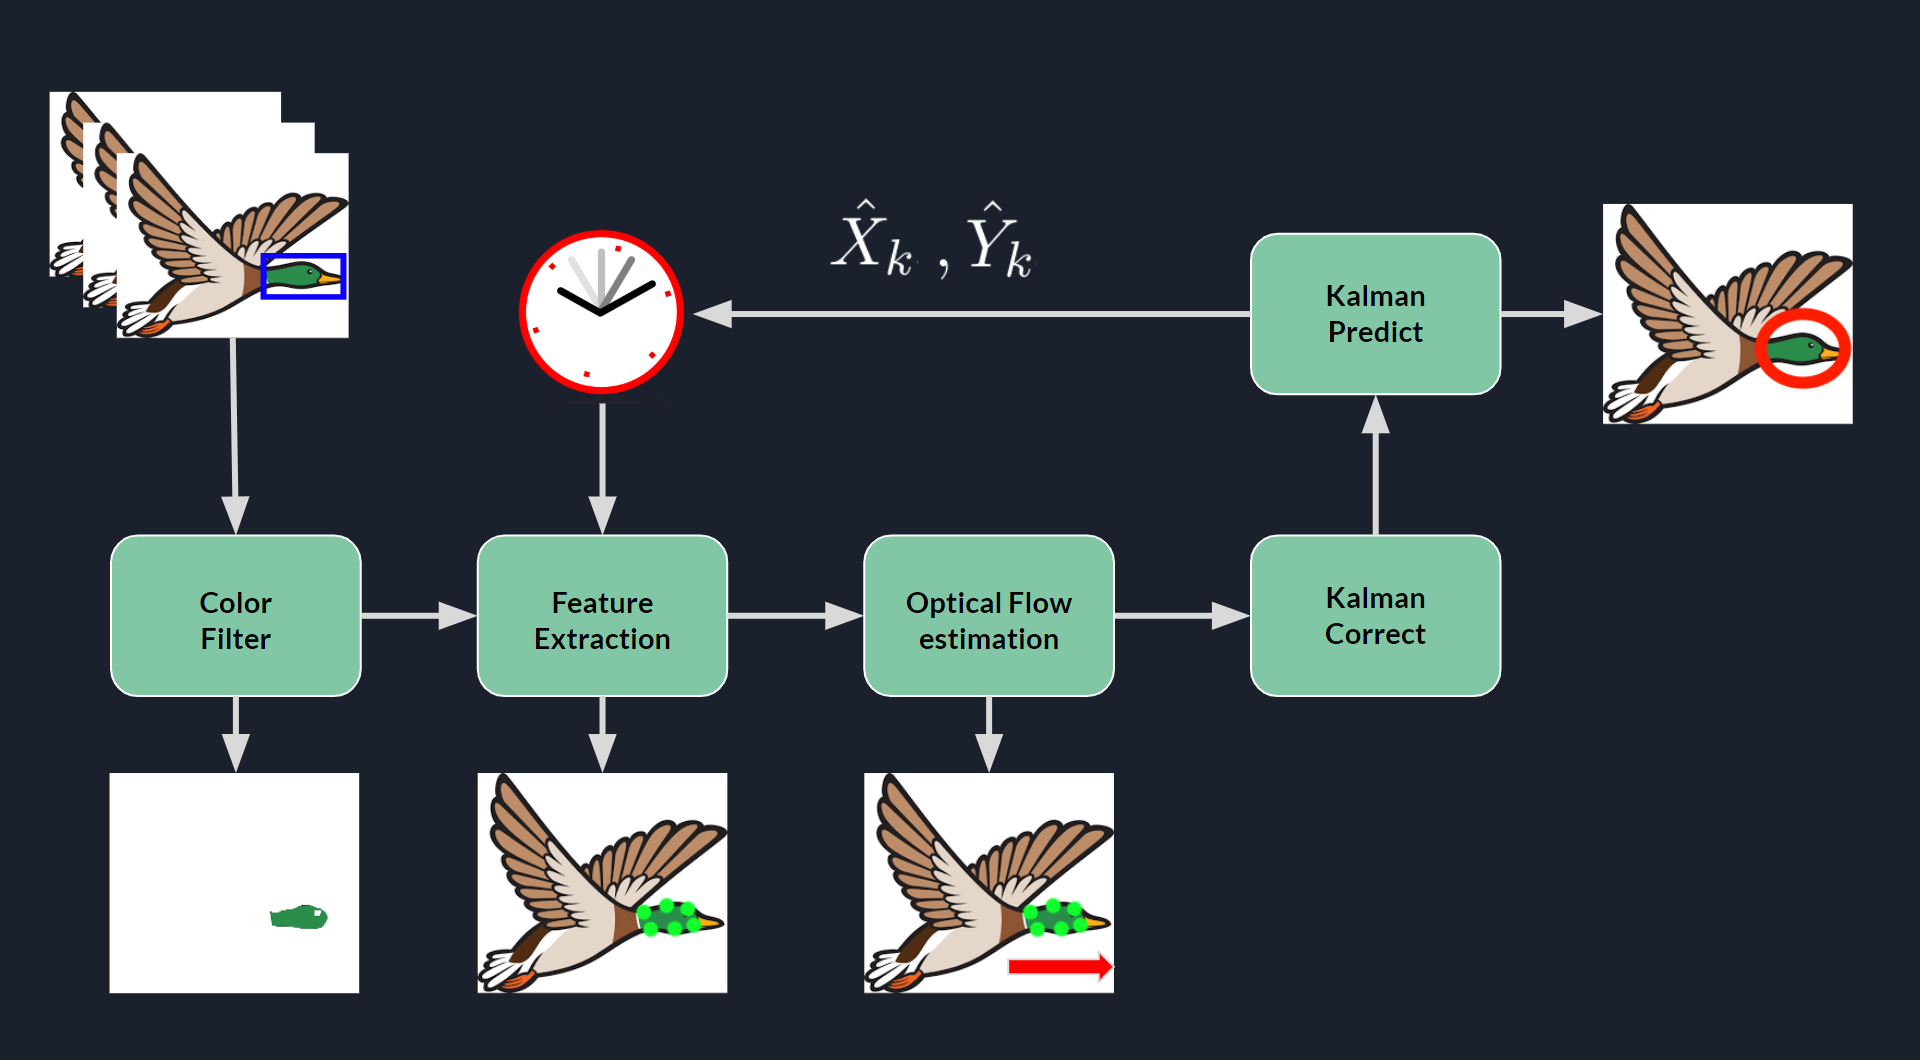
\includegraphics[width=0.5\textwidth]{Imagenes/diagram.png}
%	\caption{Diagrama en bloques del programa.}
%	\label{fig:bloques}
%\end{figure}

\subsection{Escenarios de fallas}
Si bien se han minimizado las probabilidades de cometer errores de tipo I y tipo II, aún se plantean los siguientes problemas:
\begin{itemize}
%\item En caso de oclusión del objeto de interés $A$ y en la presencia de otro objeto de cualidades similares $B$ el algoritmo podrá dar un falso positivo.
%\item El cambio de trayectoria de un objeto ocluido provocará una falla en la predicción de la trayectoria, si bien a diferencia del diseño anterior, ahora no habrá problemas en retornar al objeto correcto una vez que vuelva a aparecer en pantalla.
\item El algoritmo se encuentra en su situación más frágil al haber un objecto idéntico o de gran similaridad tanto en color como en forma con el que se quiere seguir, debido a que ni el filtro de distribución de color ni el filtro de correlación lograrán distinguir entre ambos. En este caso la única distinción entre ambos será la retención de esquinas características al objeto correcto proporcionado por el algoritmo de Optical Flow. 
\item La correcta elección de parámetros de los algoritmos encargados de la fase de enmascaramiento para cada situación proporcionan una gran robustez frente a cambios en la iluminación. Sin embargo, cuanto más robusto frente a cambios en la iluminación es el algoritmo, mayor será la probabilidad de cometer errores del tipo II (seguir a un objeto incorrecto) debido a que el enmascaramiento tendrá una mayor permisividad. 
\end{itemize}



